\documentclass[12pt,oneside,a4paper,article]{abntex2}
\usepackage[utf8]{inputenc}
\usepackage[T1]{fontenc}
\usepackage[brazil]{babel}
\usepackage{graphicx}
\usepackage{tabularx}
\usepackage{amsmath}
\usepackage{authblk}
\usepackage{float}
\usepackage{booktabs}
\usepackage{xcolor}
\usepackage{listings}

\usepackage[alf]{abntex2cite}

\usepackage[left=3cm,right=2cm,top=3cm,bottom=2cm]{geometry}
\usepackage{setspace}

\title{\textbf{FinFamily: Sistema de Gestão Financeira e Controle de Investimentos Familiar -- Implementação da Unidade II}}
\author{Matheus Ramos de Oliveira \thanks{matheusramos.oliveira@ucsal.edu.br}}
\author{Alexandre Villarino e Silva \thanks{alexandrevillarino.silva@ucsal.edu.br}}
\author[1]{Eduardo Rocha Santos \thanks{eduardorocha.santos@ucsal.edu.br}}
\author[1]{Daniel Teixeira Melo \thanks{danielteixeira.melo@ucsal.edu.br}}
\author[1]{Marcos Vinicius Sousa Batista \thanks{marcos.batista@ucsal.edu.br}}
\author[1]{Vinicius Freitas de Oliveira Souza \thanks{viniciusfreitas.souza@ucsal.edu.br}}
\author[1*]{Elton Figueiredo da Silva \thanks{elton.figueiredo@pro.ucsal.edu.br}}

\affil{
  Bacharelado em Engenharia de Software \par
  Escola de Tecnologias \par
Universidade Católica do Salvador (UCSAL) \par
Av. Prof. Pinto de Aguiar, 2589 Pituaçu, CEP: 41740-090 \par
Salvador/BA, Brasil
}
\affil[1]{\textit {\{matheusramos.oliveira, alexandrevillarino.silva, eduardorocha.santos, danielteixeira.melo, marcos.batista, viniciusfreitas.souza\}@ucsal.edu.br}}
\affil[1*]{\textit {elton.figueiredo@pro.ucsal.edu.br}}

\date{Novembro 2026}

\ifthenelse{\equal{\ABNTEXisarticle}{true}}{%
\renewcommand{\maketitlehookb}{}
}{}

\hypersetup{
      colorlinks=false,
      pdfborder={0 0 0},
}

\renewcommand*{\Authsep}{, }
\renewcommand*{\Authand}{, }
\renewcommand*{\Authands}{, }
\renewcommand*{\Affilfont}{\normalsize\normalfont}
\renewcommand*{\Authfont}{\bfseries}
\setlength{\affilsep}{2em}

\newsavebox\affbox

\renewcommand{\lstlistingname}{Código}
\lstset{
    language=Java,
    basicstyle=\ttfamily\footnotesize,
    keywordstyle=\color{blue!70!black}\bfseries,
    commentstyle=\color{green!45!black}\itshape,
    stringstyle=\color{red!60!black},
    numbers=left,
    numberstyle=\tiny\color{gray},
    numbersep=6pt,
    frame=single,
    rulecolor=\color{gray!50},
    breaklines=true,
    breakatwhitespace=true,
    tabsize=2,
    showstringspaces=false,
    extendedchars=true,
    literate={á}{{\'a}}1 {ã}{{\~a}}1 {â}{{\^a}}1 {é}{{\'e}}1 {ê}{{\^e}}1 {í}{{\'i}}1 {ó}{{\'o}}1 {õ}{{\~o}}1 {ú}{{\'u}}1 {ç}{{\c{c}}}1
}

\begin{document}

\begin{center}
    
\includegraphics[width=0.3\textwidth]{imagens-template/ucsal_logo.png}
\end{center}
{\let\newpage\relax\maketitle}

\begin{resumoumacoluna}
Este artigo apresenta a implementação da Unidade II do FinFamily, sistema web de gestão financeira e controle de investimentos familiar especificado na Unidade I. O sistema foi construído em três camadas, com Java 21 e Spring Boot 3.3.5 no servidor, React 18 e TailwindCSS na interface e banco de dados relacional H2/PostgreSQL. São apresentados o repositório versionado, o Modelo C4 nos níveis de contexto, contêineres, componentes e código, as telas do front-end em execução e os principais trechos do código do back-end. O assistente conversacional (RF-012) envia o comando do usuário a um modelo de linguagem (Google Gemini ou Ollama local) e utiliza um motor local apenas como contingência. O acesso é controlado por perfil no servidor, de modo que Titular, Membro, Auditor e Administrador do Sistema executam apenas as operações previstas na especificação. Os doze requisitos funcionais, as seis regras de negócio e o controle de acesso foram verificados por 33 testes automatizados.
 \vspace{\onelineskip}

 \noindent
 \textbf{Palavras-chaves}: gestão financeira, Spring Boot, React, Modelo C4, inteligência artificial.
\end{resumoumacoluna}

\renewcommand{\resumoname}{Abstract}
\begin{resumoumacoluna}
This paper presents the second-unit implementation of FinFamily, a web system for family financial management and investment tracking specified in the first unit. The system follows a three-layer architecture with Java 21 and Spring Boot 3.3.5 on the server, React 18 and TailwindCSS on the user interface, and an H2/PostgreSQL relational database. It describes the version-controlled repository, the C4 model at the context, container, component and code levels, the running front-end screens and the main back-end source code. The conversational assistant (RF-012) sends the user's command to a large language model (Google Gemini or a local Ollama model) and uses a local engine only as a fallback. Access control is enforced on the server by user role, so that each profile performs only the operations defined in the specification. The twelve functional requirements, the six business rules and the access control were verified by 33 automated tests.
 \vspace{\onelineskip}

 \noindent
 \textbf{Keywords}: financial management, Spring Boot, React, C4 model, artificial intelligence.
\end{resumoumacoluna}

\textual

\section{Introdução}

Na Unidade I foram especificados o problema da dispersão das informações financeiras das famílias, os objetivos específicos (OE1 a OE6), os doze requisitos funcionais (RF-001 a RF-012), as seis regras de negócio (RN-001 a RN-006), os sete requisitos não funcionais (RNF-001 a RNF-007), os fluxos de processo em BPMN \cite{omg2014}, o diagrama de classes e o diagrama de casos de uso em UML \cite{omg2017}, seguindo os princípios de engenharia de requisitos de \citeonline{sommerville2019} e \citeonline{pressman2021}.

Este artigo documenta a Unidade II, dedicada à implementação, e está organizado conforme os itens do roteiro do trabalho semestral: o repositório versionado (Item 11, Seção \ref{sec:repositorio}), o Modelo C4 (Item 12, Seção \ref{sec:c4}), as telas do front-end (Item 13, Seção \ref{sec:telas}), o código do back-end (Item 14, Seção \ref{sec:codigo}) e os vídeos individuais (Item 15, Seção \ref{sec:videos}). A Seção \ref{sec:gestao} descreve a gestão do projeto e a Seção \ref{sec:validacao}, a verificação dos resultados.

\section{Gestão do Projeto}
\label{sec:gestao}

O projeto foi conduzido com o framework Scrum \cite{schwaber2020}, em quatro sprints de duas semanas, conforme o cronograma da Unidade I. As tarefas foram acompanhadas em um quadro Kanban no Trello, disponível em \url{https://trello.com/b/EwMCmp64}. Os papéis da equipe foram distribuídos da seguinte forma: ScrumMaster, Matheus Ramos de Oliveira; e desenvolvedores, Alexandre Villarino e Silva, Daniel Teixeira Melo, Eduardo Rocha Santos, Marcos Vinicius Sousa Batista e Vinicius Freitas de Oliveira Souza.

O código foi versionado com Git no GitHub, na branch principal (\textit{main}). A integração com o modelo de linguagem e o controle de acesso por perfil foram desenvolvidos na branch \textit{feat/ia-e-controle-de-acesso} e incorporados à branch principal por meio de \textit{pull request}, o que deixa registrado no repositório o histórico de contribuições da equipe.

\section{Repositório Versionado e Tecnologias (Item 11)}
\label{sec:repositorio}

O código-fonte e os artefatos do projeto estão versionados com Git no repositório \url{https://github.com/d3vPadawann/proj_topicos_avancados}, organizado nas seguintes pastas:

\begin{itemize}
    \item \texttt{backend/}: servidor em Java 21 com Spring Boot 3.3.5 \cite{spring2024}, Spring Data JPA, Spring Security, jjwt, OpenPDF, Apache POI e testes em JUnit 5; inclui o Maven Wrapper (\texttt{mvnw.cmd}), que dispensa a instalação do Maven;
    \item \texttt{frontend/}: aplicação de página única em React 18, Vite e TailwindCSS, com reconhecimento de voz pela \textit{Web Speech API};
    \item \texttt{docs/}: diagramas do Modelo C4 e capturas das telas;
    \item \texttt{overleaf/}: código-fonte deste artigo;
    \item \texttt{INICIAR\_FINFAMILY.bat}: inicia o sistema em qualquer computador com JDK 21.
\end{itemize}

A Tabela \ref{tab:tecnologias} resume as decisões tecnológicas e os requisitos que cada uma atende.

\begin{table}[H]
\centering
\caption{Decisões tecnológicas da Unidade II}
\label{tab:tecnologias}
\begin{tabularx}{\textwidth}{p{3.4cm}Xp{4.2cm}}
\toprule
\textbf{Camada} & \textbf{Tecnologia} & \textbf{Requisitos} \\
\midrule
Back-end & Java 21 e Spring Boot 3.3.5 & Roteiro; RF-001 a RF-012 \\
Front-end & React 18, Vite e TailwindCSS & Roteiro; RNF-005 \\
Persistência & Spring Data JPA com H2 ou PostgreSQL & Seção 2.5 da Unidade I \\
Segurança & Spring Security, JWT, BCrypt, AES-256-GCM e regras de acesso por perfil & RF-001, OE4, RNF-003, RNF-004 \\
Inteligência artificial & Google Gemini \cite{google2026} ou Ollama local, com motor local de contingência & RF-012, RN-006, RNF-004, OE5 \\
Exportação & OpenPDF, Apache POI e CSV & RF-010 \\
Cache e agendamento & Spring Cache e \texttt{@Scheduled} & RNF-001, RNF-002, RF-011, RNF-007 \\
\bottomrule
\end{tabularx}
\fonte{Autoria própria (2026).}
\end{table}

\section{Modelo C4 (Item 12)}
\label{sec:c4}

O Modelo C4 \cite{brown2018} descreve a arquitetura em quatro níveis de abstração: contexto, contêineres, componentes e código.

O diagrama de contexto (Figura \ref{fig:c4-1}) apresenta o FinFamily e suas interações com os quatro perfis de usuário definidos na Seção 2.9 da Unidade I e com o serviço externo de inteligência artificial, que recebe apenas o texto do comando e os nomes das contas e categorias (RNF-004).

\begin{figure}[H]
    \centering
    \caption{Modelo C4 -- Nível 1: diagrama de contexto}
    \label{fig:c4-1}
    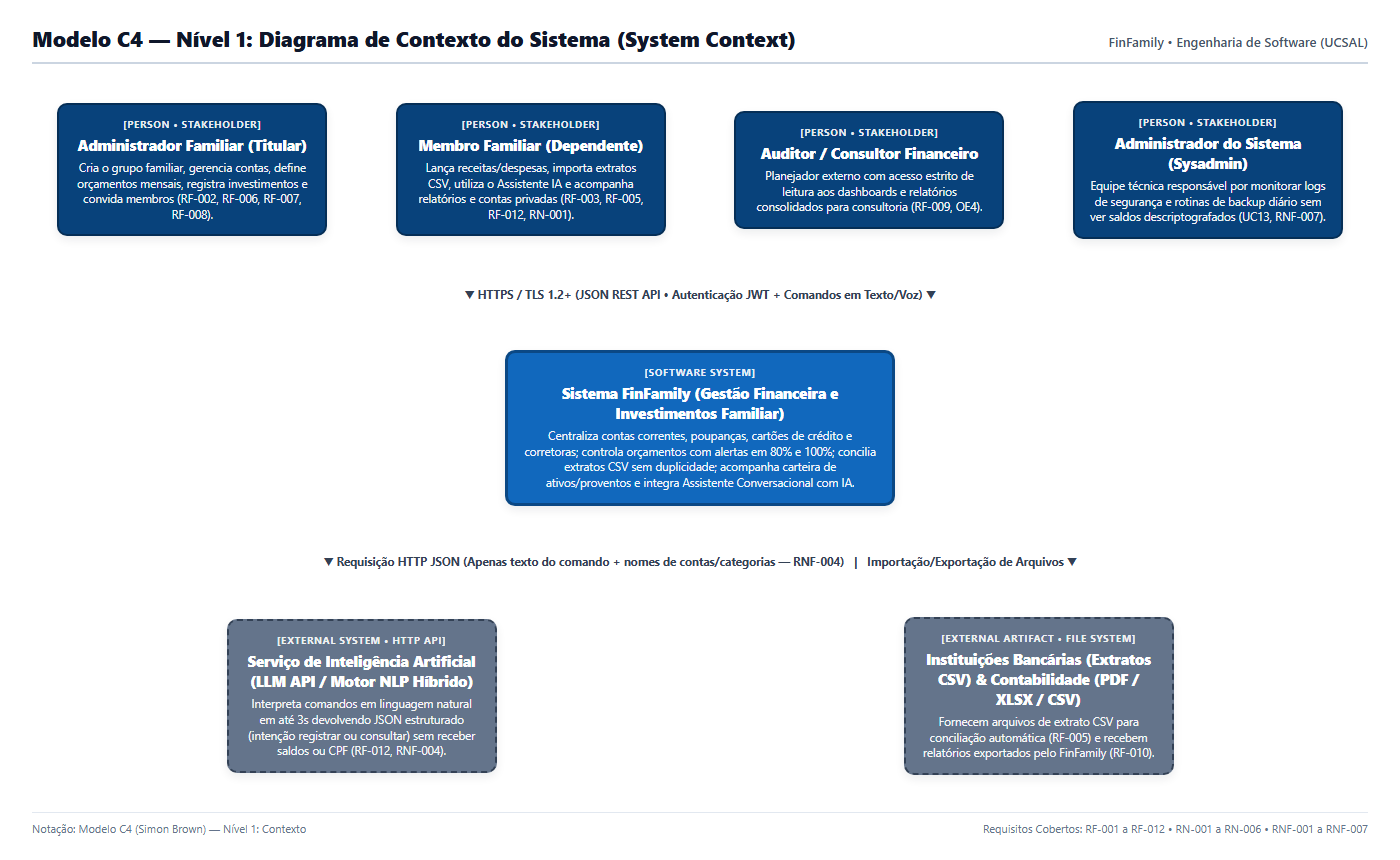
\includegraphics[width=\textwidth]{figuras/c4_nivel1_contexto.png}
    \fonte{Autoria própria (2026).}
\end{figure}

O diagrama de contêineres (Figura \ref{fig:c4-2}) detalha a arquitetura em três camadas da Seção 2.5 da Unidade I: a interface web executada no navegador, o servidor de aplicação com a API REST e o banco de dados relacional, além do armazenamento de backups diários (RNF-007).

\begin{figure}[H]
    \centering
    \caption{Modelo C4 -- Nível 2: diagrama de contêineres}
    \label{fig:c4-2}
    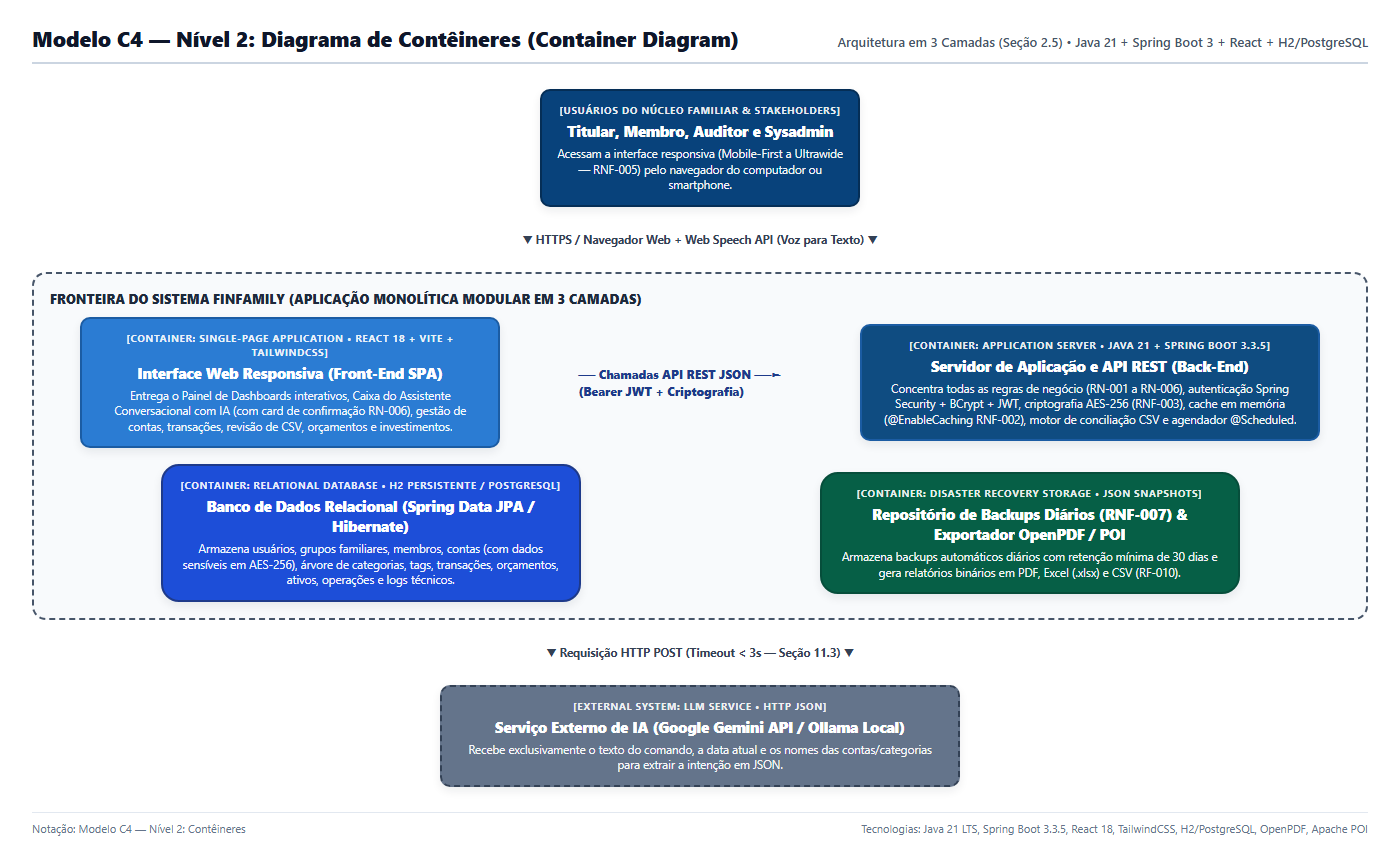
\includegraphics[width=\textwidth]{figuras/c4_nivel2_conteineres.png}
    \fonte{Autoria própria (2026).}
\end{figure}

O diagrama de componentes (Figura \ref{fig:c4-3}) mostra a divisão interna do servidor: os controladores REST; os componentes de segurança (\texttt{SecurityConfig}, com as regras por perfil; \texttt{JwtAuthenticationFilter} e \texttt{JwtTokenProvider}, que validam o token; \texttt{ControleAcesso}, que verifica se cada registro pertence ao grupo do usuário; e \texttt{AesAttributeConverter}); os serviços de domínio, entre eles o \texttt{AssistenteIAService} e o \texttt{ClienteLLM}, responsável pela comunicação com o modelo de linguagem; e os repositórios JPA.

\begin{figure}[H]
    \centering
    \caption{Modelo C4 -- Nível 3: diagrama de componentes do back-end}
    \label{fig:c4-3}
    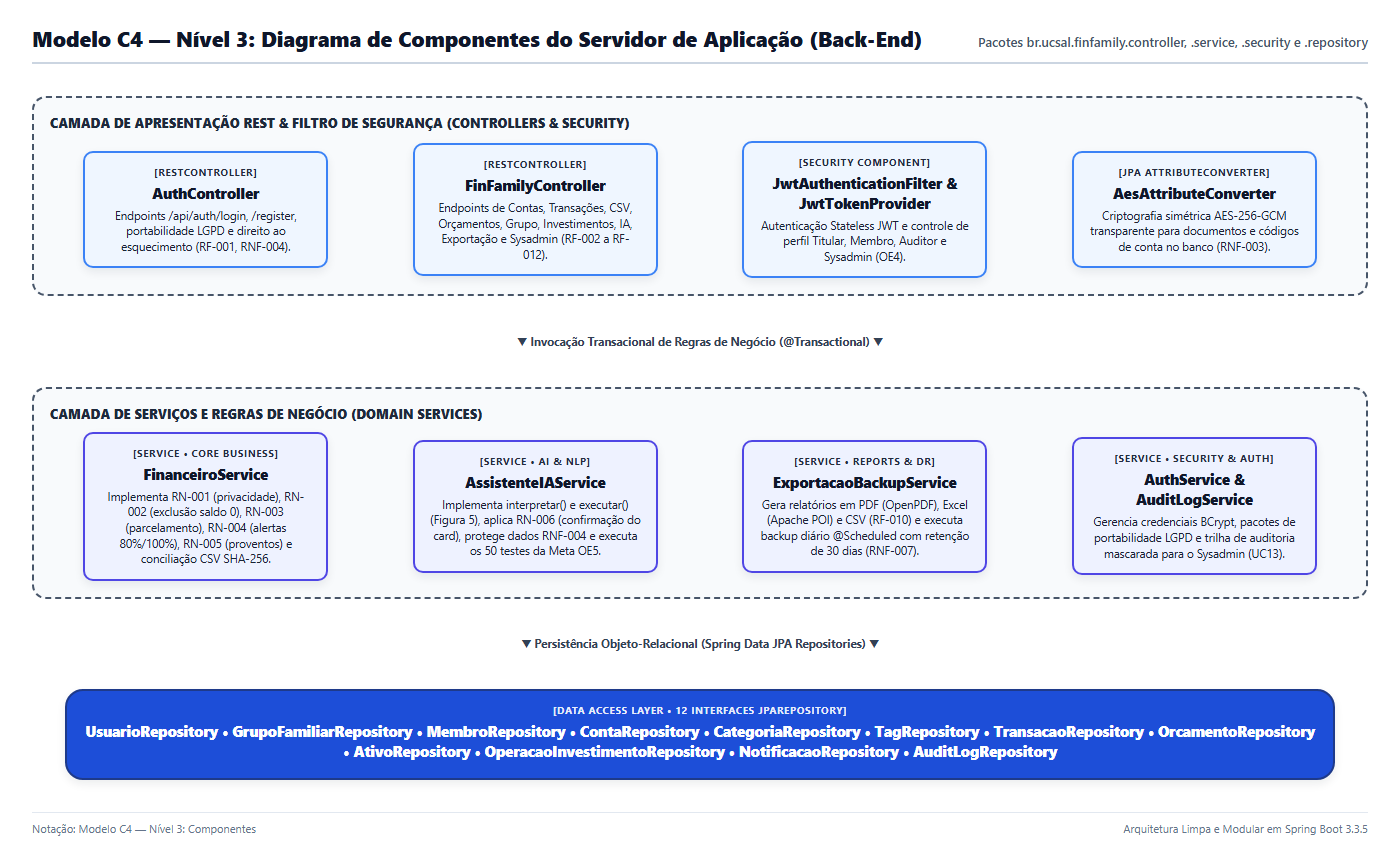
\includegraphics[width=\textwidth]{figuras/c4_nivel3_componentes.png}
    \fonte{Autoria própria (2026).}
\end{figure}

O diagrama de código (Figura \ref{fig:c4-4}) relaciona o diagrama de classes da Unidade I às classes Java implementadas no pacote \texttt{br.ucsal.finfamily.domain.model}, mantendo os atributos, as enumerações e os métodos de negócio especificados.

\begin{figure}[H]
    \centering
    \caption{Modelo C4 -- Nível 4: diagrama de código}
    \label{fig:c4-4}
    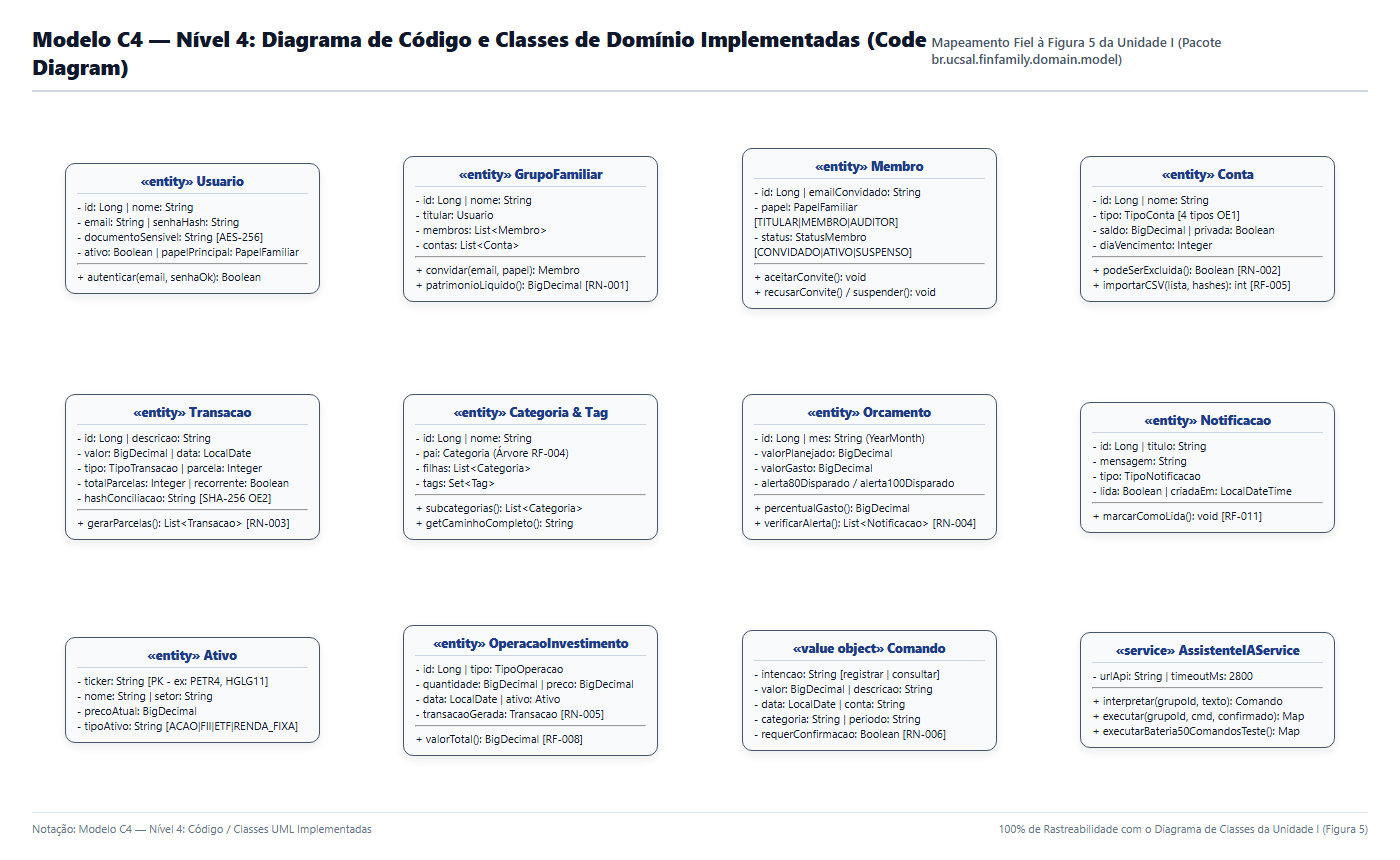
\includegraphics[width=\textwidth]{figuras/c4_nivel4_codigo.png}
    \fonte{Autoria própria (2026).}
\end{figure}

\section{Telas do Front-End (Item 13)}
\label{sec:telas}

A interface foi desenvolvida em React com TailwindCSS, no padrão \textit{mobile-first} (RNF-005). As figuras desta seção são capturas da aplicação em execução, integrada ao servidor.

\subsection{Autenticação}

O sistema abre na tela de autenticação (Figura \ref{fig:login}) e não exibe dados sem login. O usuário informa e-mail e senha, verificada por \textit{hash} BCrypt, e recebe um token JWT. Os botões dos perfis de demonstração apenas preenchem o e-mail; a senha é sempre exigida. A sessão é mantida separadamente em cada aba do navegador.

\begin{figure}[H]
    \centering
    \caption{Tela de autenticação (RF-001)}
    \label{fig:login}
    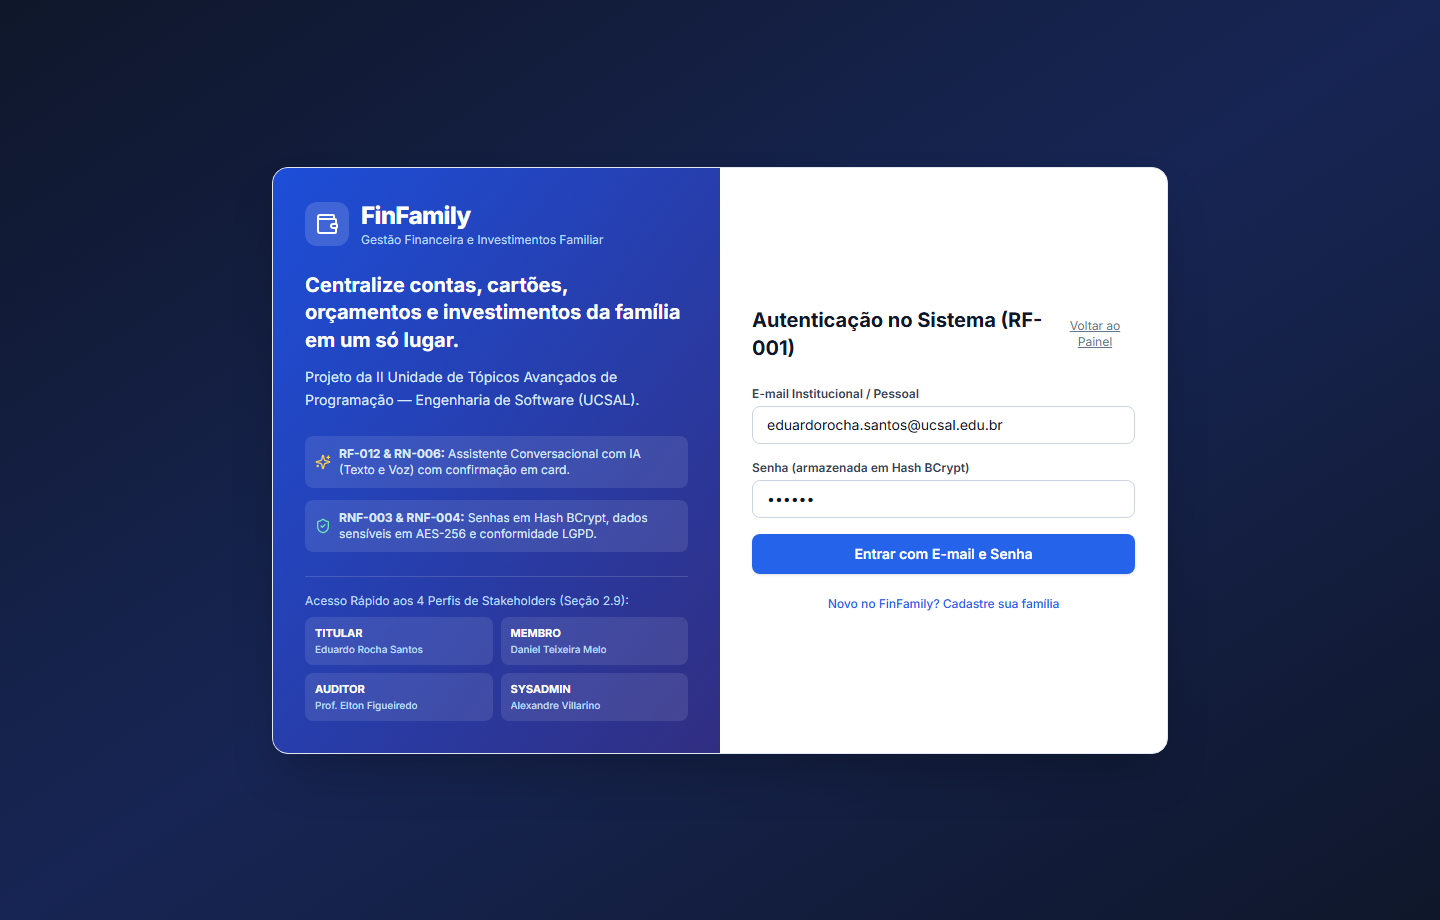
\includegraphics[width=0.95\textwidth]{figuras/tela_01_login.png}
    \fonte{Autoria própria (2026).}
\end{figure}

\subsection{Painel principal e assistente conversacional}

A tela inicial (Figura \ref{fig:painel}) reúne o assistente conversacional (RF-012), que aceita texto ou voz. Ao receber o comando ``Registrar gasto de R\$ 45,90 na padaria hoje no cartão de crédito'', o sistema envia o texto ao modelo de linguagem, que devolve a intenção e os campos em JSON. O sistema então exibe o card de confirmação editável, que indica o serviço e o modelo utilizados; nada é gravado sem a confirmação do usuário (RN-006). Abaixo do assistente ficam o patrimônio líquido familiar, que desconsidera as contas privadas (RN-001), a evolução patrimonial e o acompanhamento dos orçamentos.

\begin{figure}[H]
    \centering
    \caption{Painel principal e card de confirmação montado pelo Google Gemini (RF-009, RF-012, RN-006)}
    \label{fig:painel}
    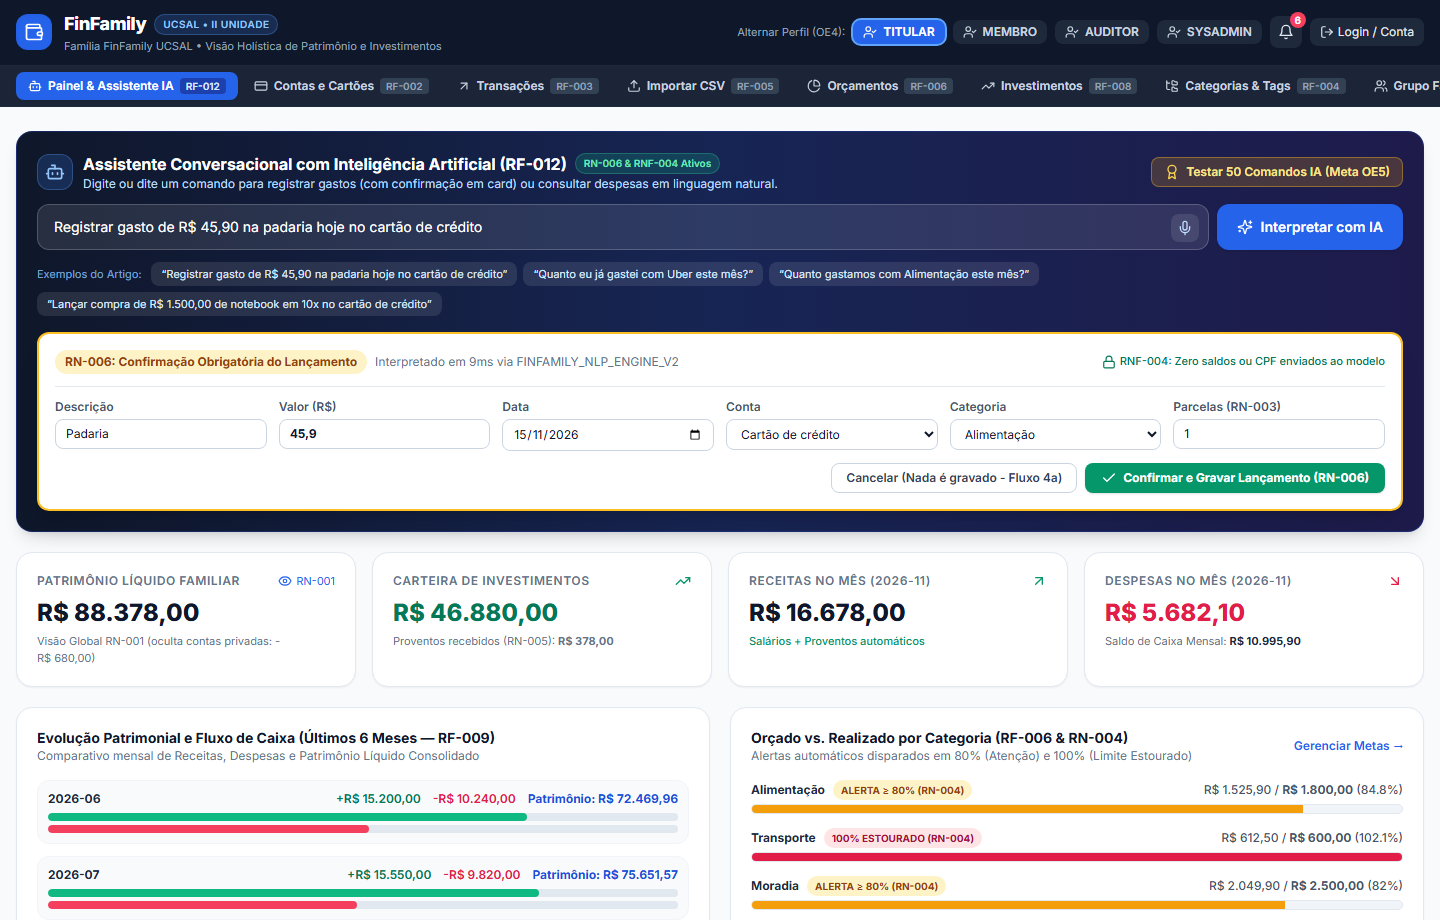
\includegraphics[width=0.95\textwidth]{figuras/tela_02_dashboard_ia.png}
    \fonte{Autoria própria (2026).}
\end{figure}

\subsection{Bateria de 50 comandos de teste (OE5)}

Conforme a Seção 11.4 da Unidade I, o sistema executa 50 comandos de teste em linguagem natural, sendo 25 de registro e 25 de consulta, e informa para cada um o resultado, o tempo e o serviço que o interpretou (Figura \ref{fig:benchmark}). Na execução apresentada, os 50 comandos foram interpretados corretamente, com tempo médio de 610 ms: 24 pelo Google Gemini dentro do limite de 3 segundos e 26 pelo motor local de contingência, acionado quando o serviço externo excedeu o tempo ou recusou a requisição por limite de uso do plano gratuito (Seção 11.3 da Unidade I).

\begin{figure}[H]
    \centering
    \caption{Resultado dos 50 comandos de teste do assistente (OE5)}
    \label{fig:benchmark}
    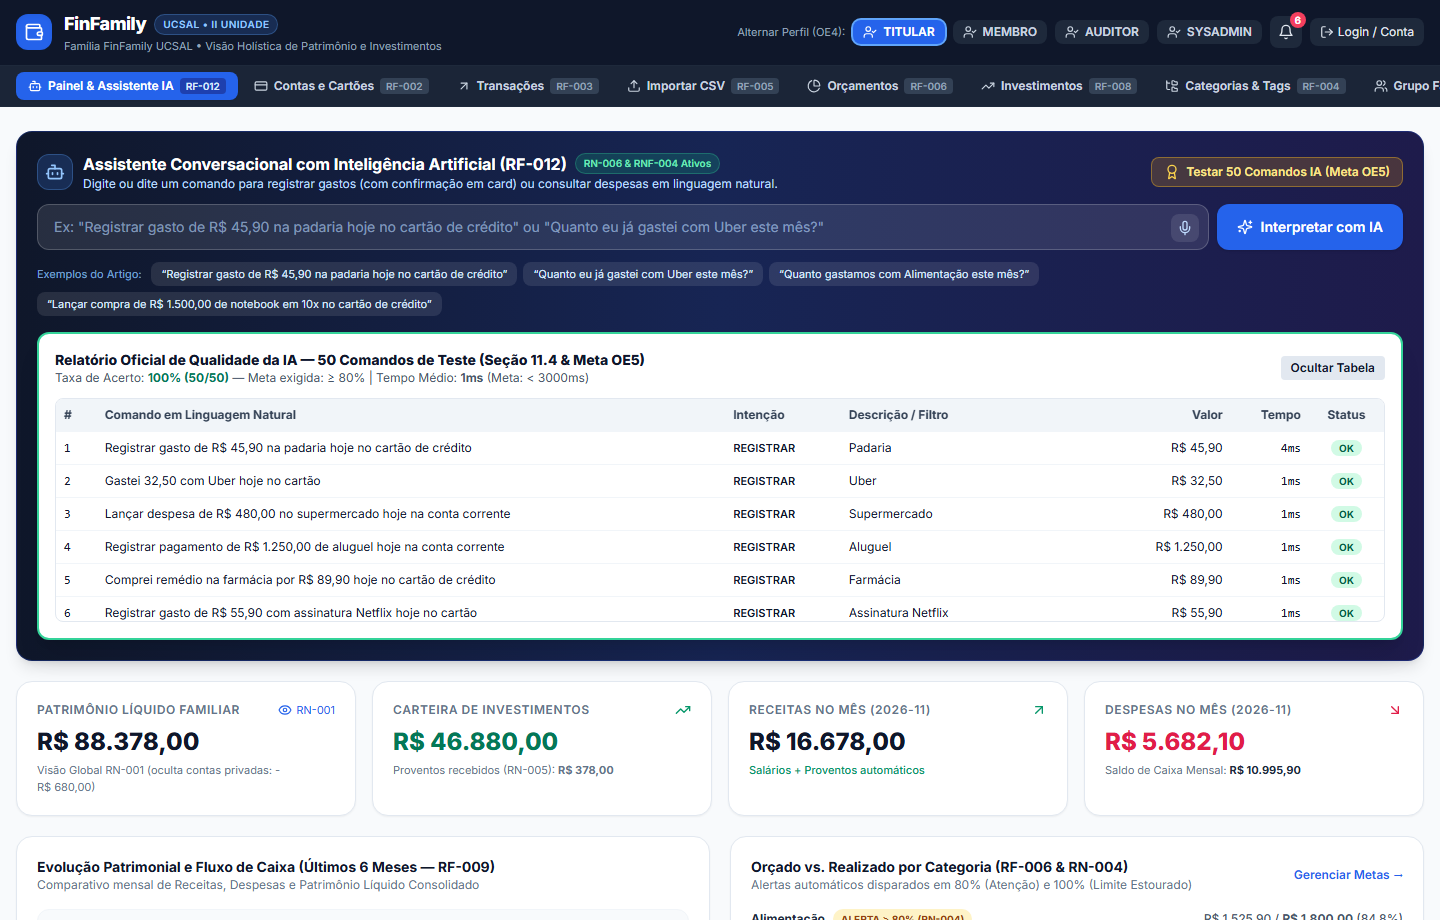
\includegraphics[width=0.95\textwidth]{figuras/tela_03_benchmark_ia_50.png}
    \fonte{Autoria própria (2026).}
\end{figure}

\subsection{Contas e cartões}

O módulo de contas (Figura \ref{fig:contas}) reúne os quatro tipos de conta da meta OE1: corrente, poupança, cartão de crédito e corretora. Contas marcadas como privadas não entram no patrimônio exibido aos demais membros (RN-001), e uma conta só pode ser excluída com saldo igual a zero (RN-002).

\begin{figure}[H]
    \centering
    \caption{Módulo de contas e cartões (RF-002, RN-001, RN-002)}
    \label{fig:contas}
    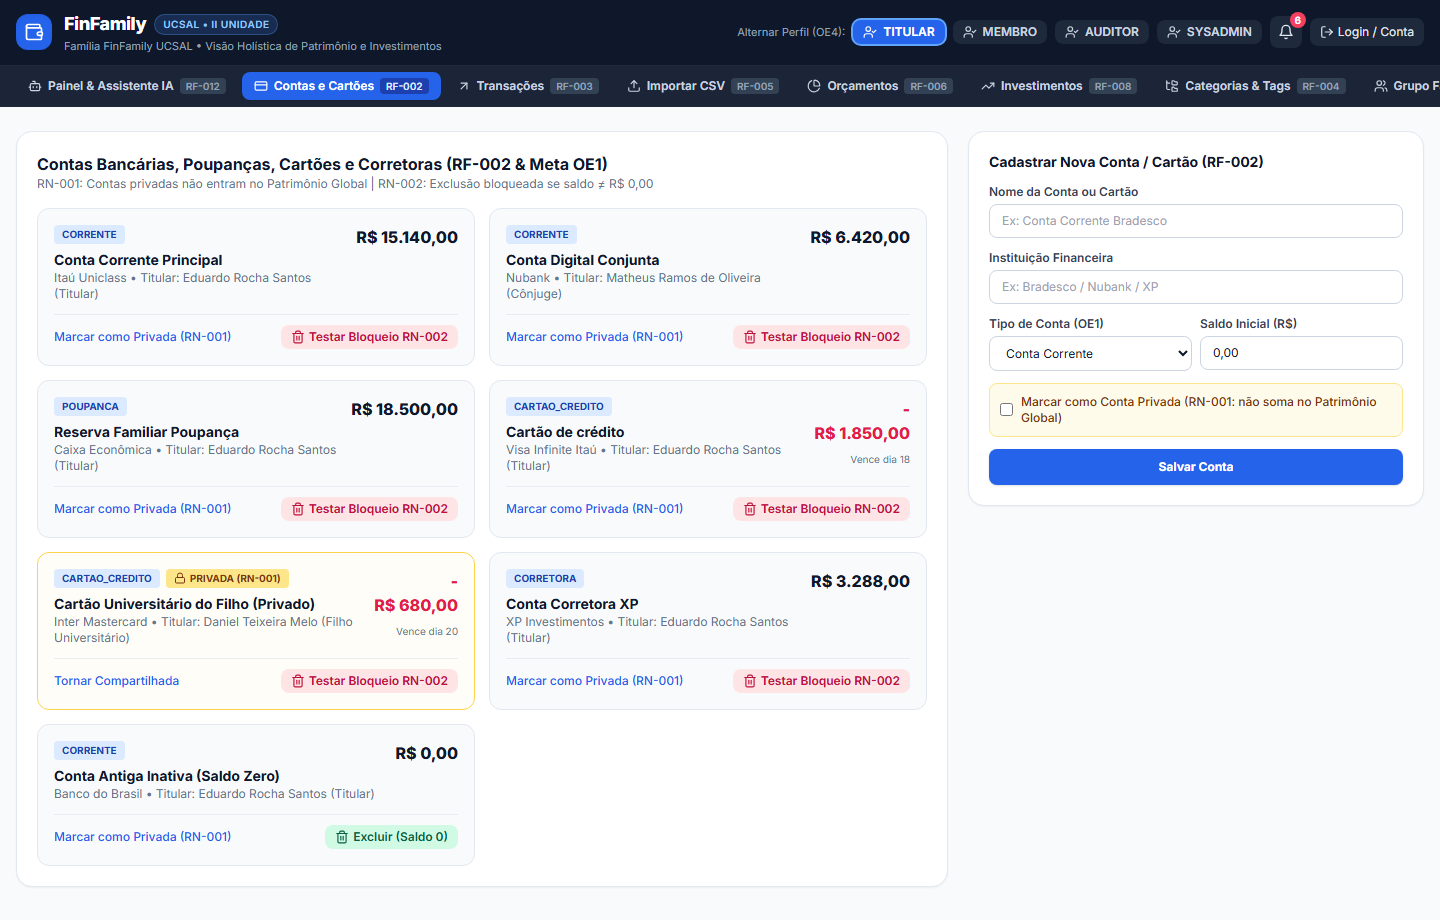
\includegraphics[width=0.95\textwidth]{figuras/tela_04_contas_cartoes.png}
    \fonte{Autoria própria (2026).}
\end{figure}

\subsection{Transações}

A tela de transações (Figura \ref{fig:transacoes}) permite registrar receitas, despesas e transferências, inclusive recorrentes, e divide automaticamente as compras parceladas, projetando as parcelas nos meses seguintes (RN-003).

\begin{figure}[H]
    \centering
    \caption{Módulo de transações com parcelamento automático (RF-003, RN-003)}
    \label{fig:transacoes}
    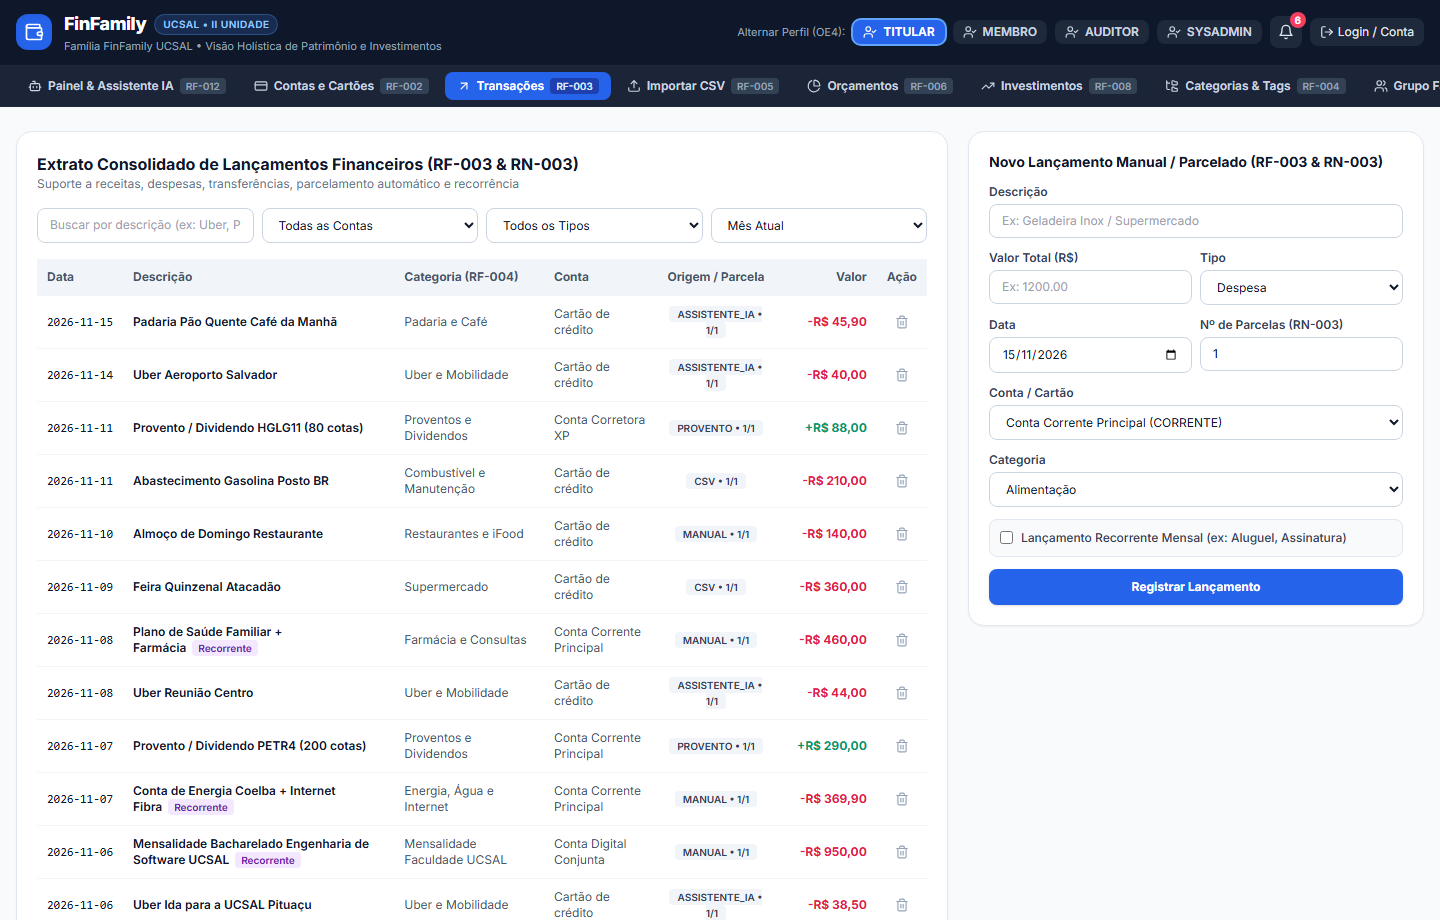
\includegraphics[width=0.95\textwidth]{figuras/tela_05_transacoes_parcelamento.png}
    \fonte{Autoria própria (2026).}
\end{figure}

\subsection{Importação de extratos CSV}

Seguindo o fluxo BPMN de importação e o caso de uso UC05, a tela de importação (Figura \ref{fig:importacao}) valida as colunas obrigatórias, descarta as linhas já importadas por meio de um \textit{hash} SHA-256 (OE2) e apresenta as transações novas para revisão das categorias antes da confirmação.

\begin{figure}[H]
    \centering
    \caption{Importação de extratos CSV sem duplicidades (RF-005, OE2)}
    \label{fig:importacao}
    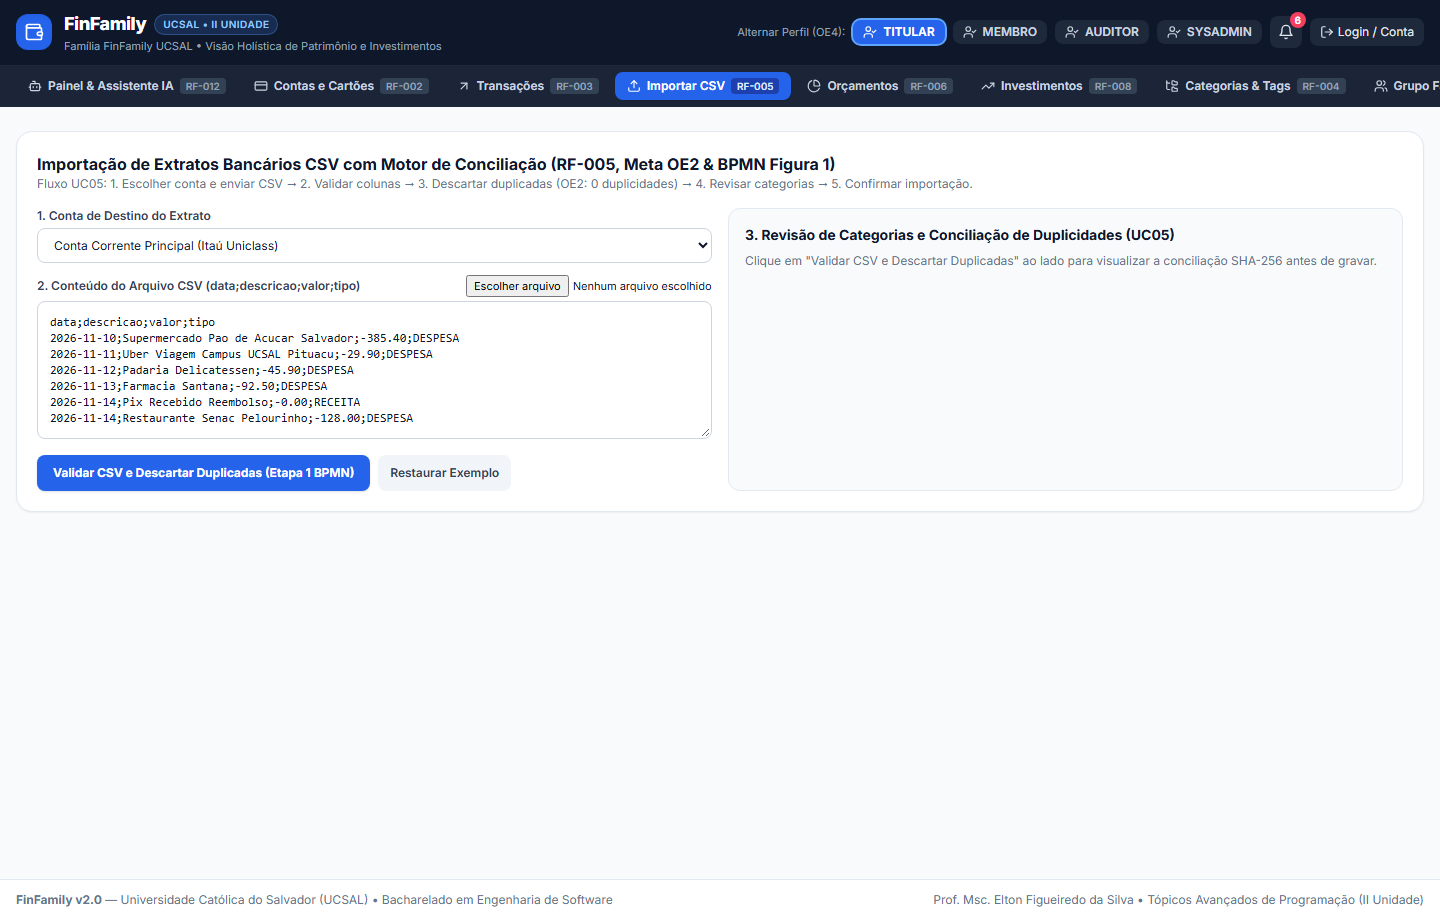
\includegraphics[width=0.95\textwidth]{figuras/tela_06_importacao_csv.png}
    \fonte{Autoria própria (2026).}
\end{figure}

\subsection{Orçamentos}

O módulo de orçamentos (Figura \ref{fig:orcamentos}) permite definir metas mensais por categoria e gera notificações quando os gastos atingem 80\% e 100\% do planejado (RN-004, OE3), como nos casos de Alimentação, com 84,8\%, e Transporte, com 102,1\%.

\begin{figure}[H]
    \centering
    \caption{Orçamentos mensais com alertas em 80\% e 100\% (RF-006, RN-004)}
    \label{fig:orcamentos}
    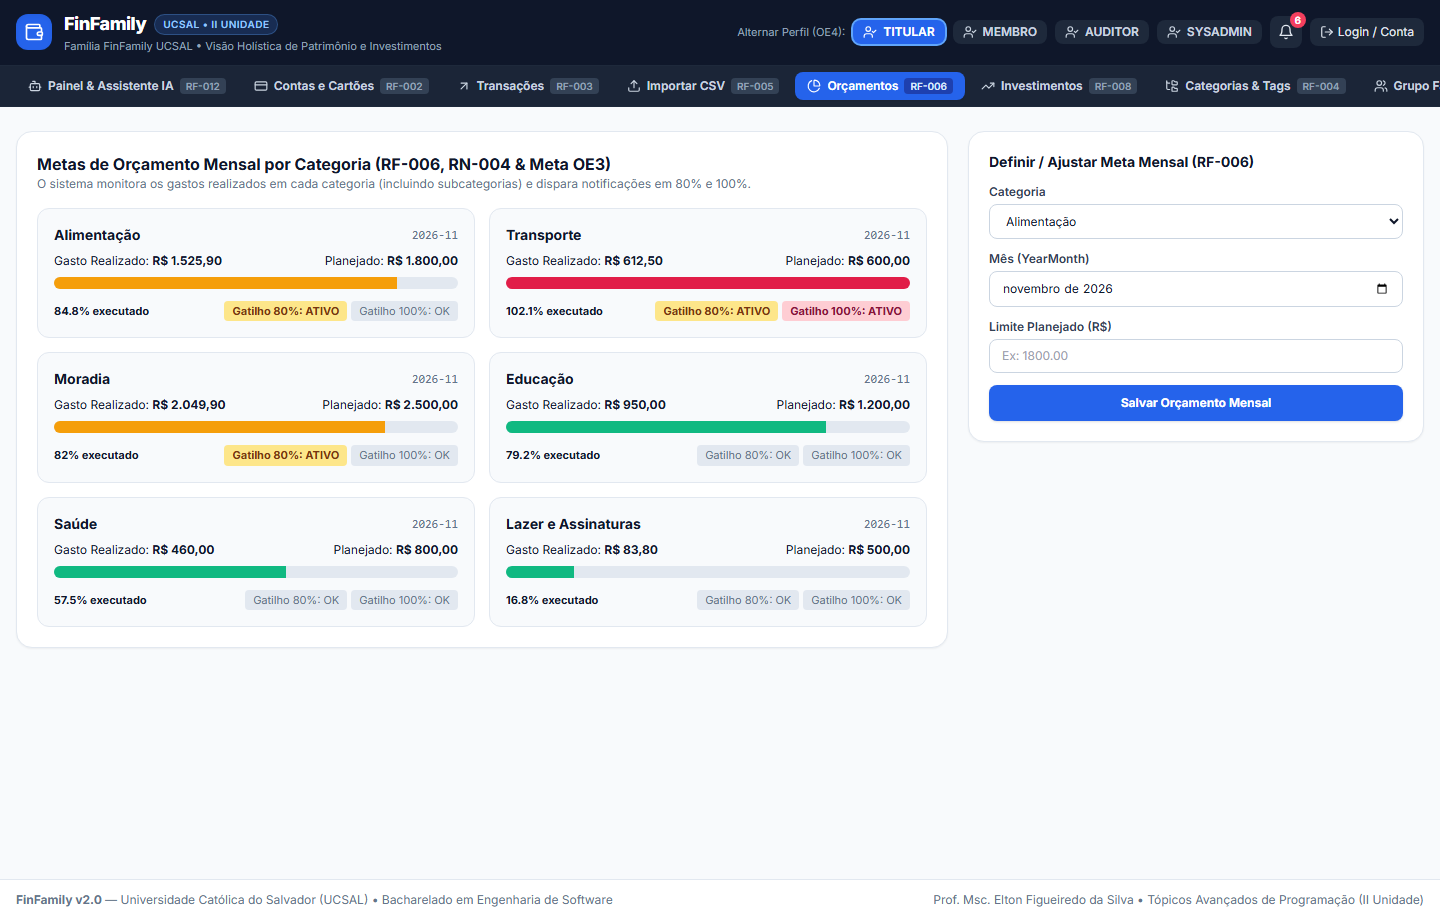
\includegraphics[width=0.95\textwidth]{figuras/tela_07_orcamentos_alertas.png}
    \fonte{Autoria própria (2026).}
\end{figure}

\subsection{Investimentos}

O módulo de investimentos (Figura \ref{fig:investimentos}) acompanha a posição por \textit{ticker}, com quantidade, preço médio, valor de mercado e rentabilidade. Cada provento registrado gera automaticamente uma receita na conta de destino (RN-005).

\begin{figure}[H]
    \centering
    \caption{Investimentos e registro de proventos como receita (RF-008, RN-005)}
    \label{fig:investimentos}
    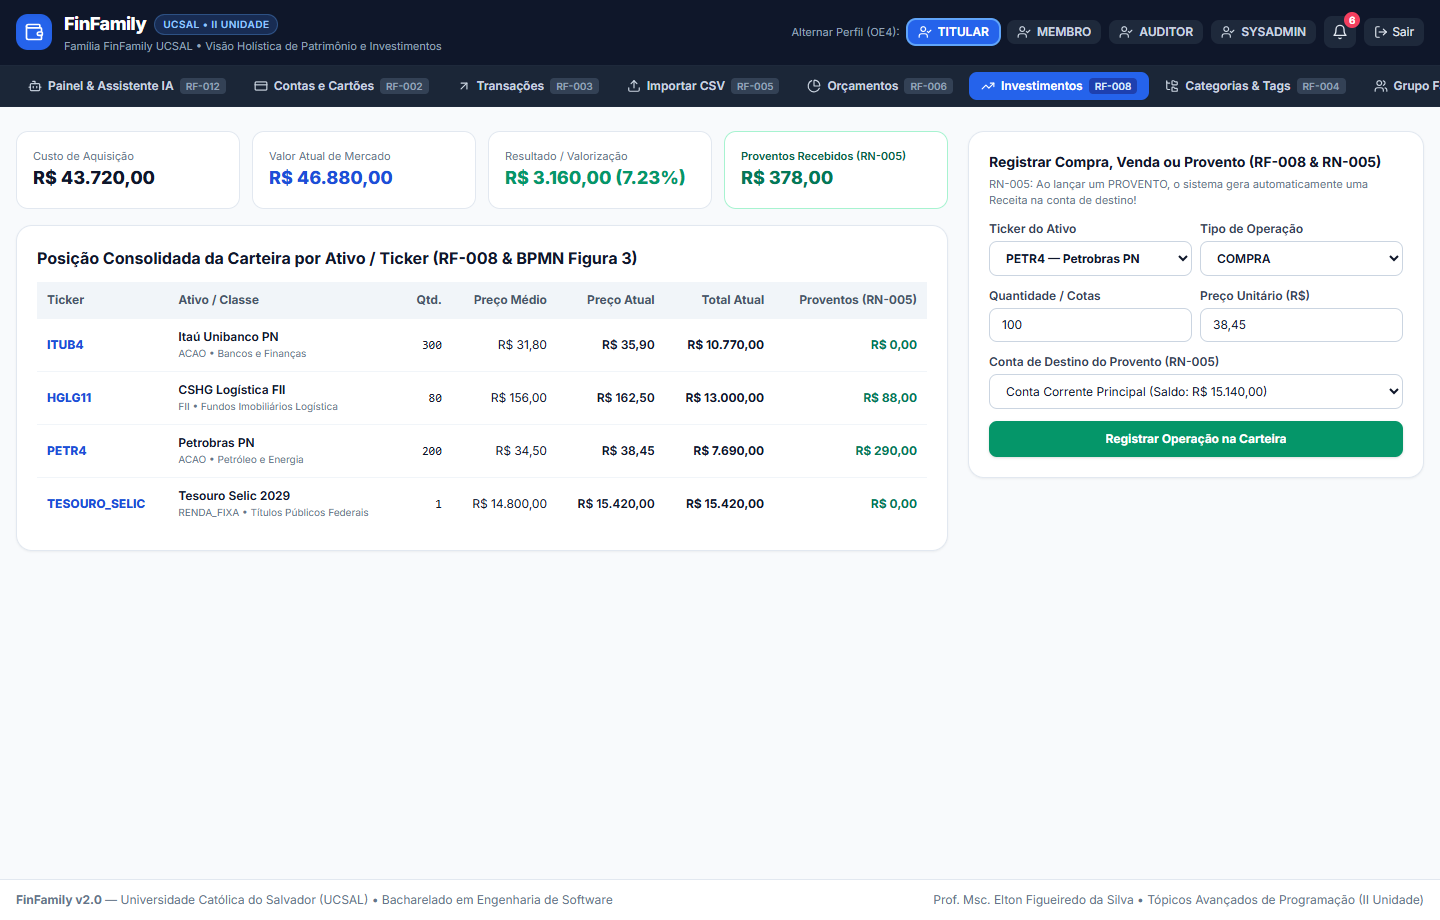
\includegraphics[width=0.95\textwidth]{figuras/tela_08_investimentos_proventos.png}
    \fonte{Autoria própria (2026).}
\end{figure}

\subsection{Grupo familiar}

A tela do grupo familiar (Figura \ref{fig:grupo}) implementa o fluxo BPMN de inclusão de membro: o Titular convida novos membros com o papel de Membro ou Auditor e pode suspendê-los ou reativá-los. A resposta ao convite é dada pelo próprio convidado, como mostra a Subseção \ref{sec:convite}.

\begin{figure}[H]
    \centering
    \caption{Gestão do grupo familiar (RF-007, OE4)}
    \label{fig:grupo}
    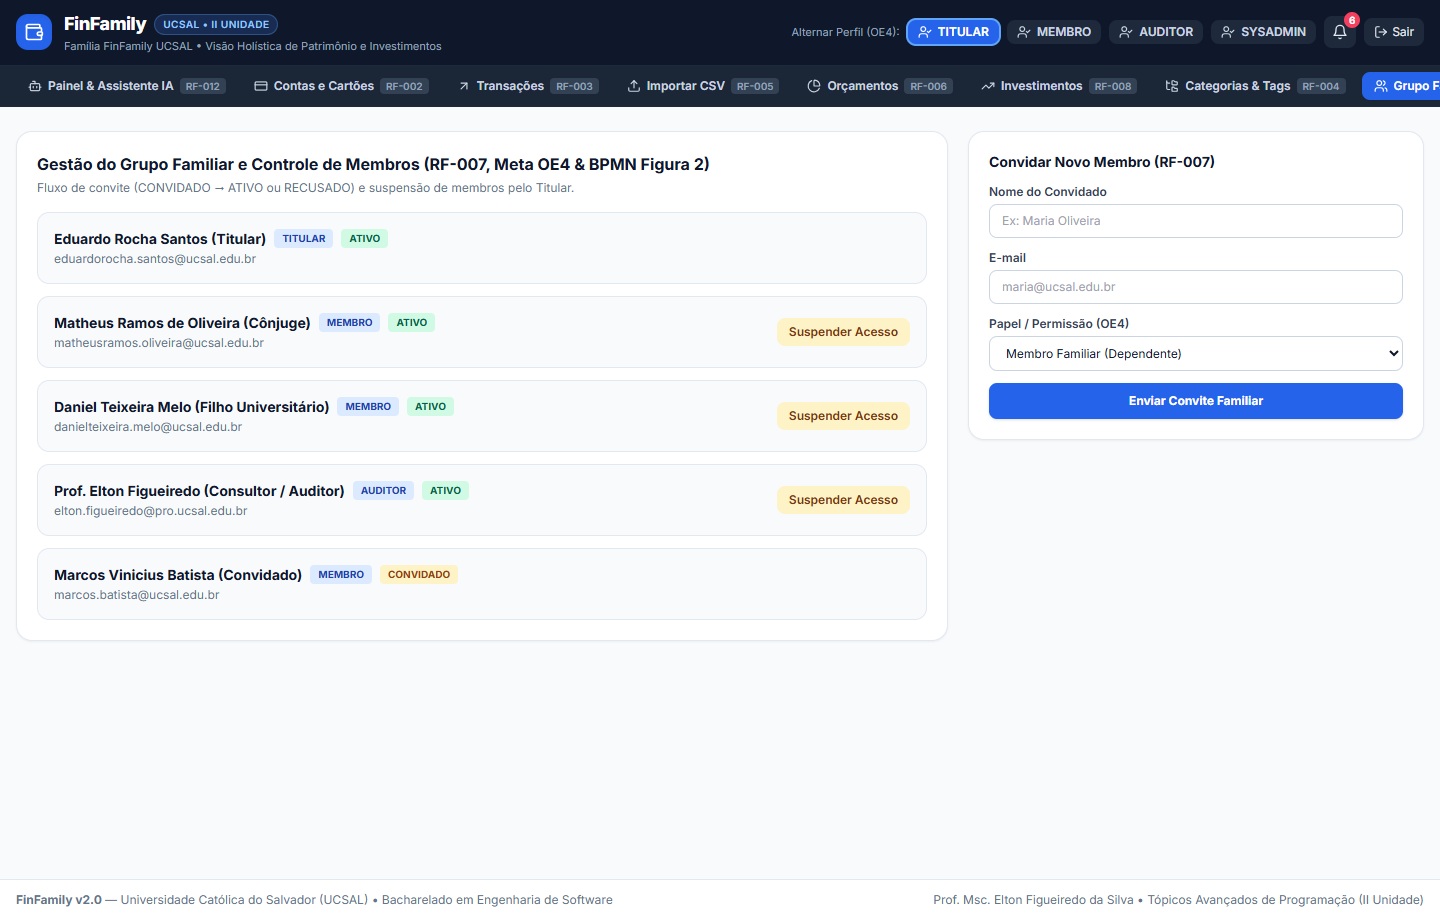
\includegraphics[width=0.95\textwidth]{figuras/tela_09_grupo_familiar.png}
    \fonte{Autoria própria (2026).}
\end{figure}

\subsection{LGPD, backup e logs}

O painel de segurança (Figura \ref{fig:seguranca}) permite ao usuário baixar os próprios dados pessoais, em conformidade com a LGPD \cite{brasil2018} e o RNF-004. Para o Administrador do Sistema, exibe a rotina de backup diário com retenção de 30 dias (RNF-007) e os logs técnicos (UC13), sem acesso aos dados financeiros.

\begin{figure}[H]
    \centering
    \caption{Painel de LGPD, backup e logs técnicos visto pelo Administrador do Sistema (RNF-004, RNF-007, UC13)}
    \label{fig:seguranca}
    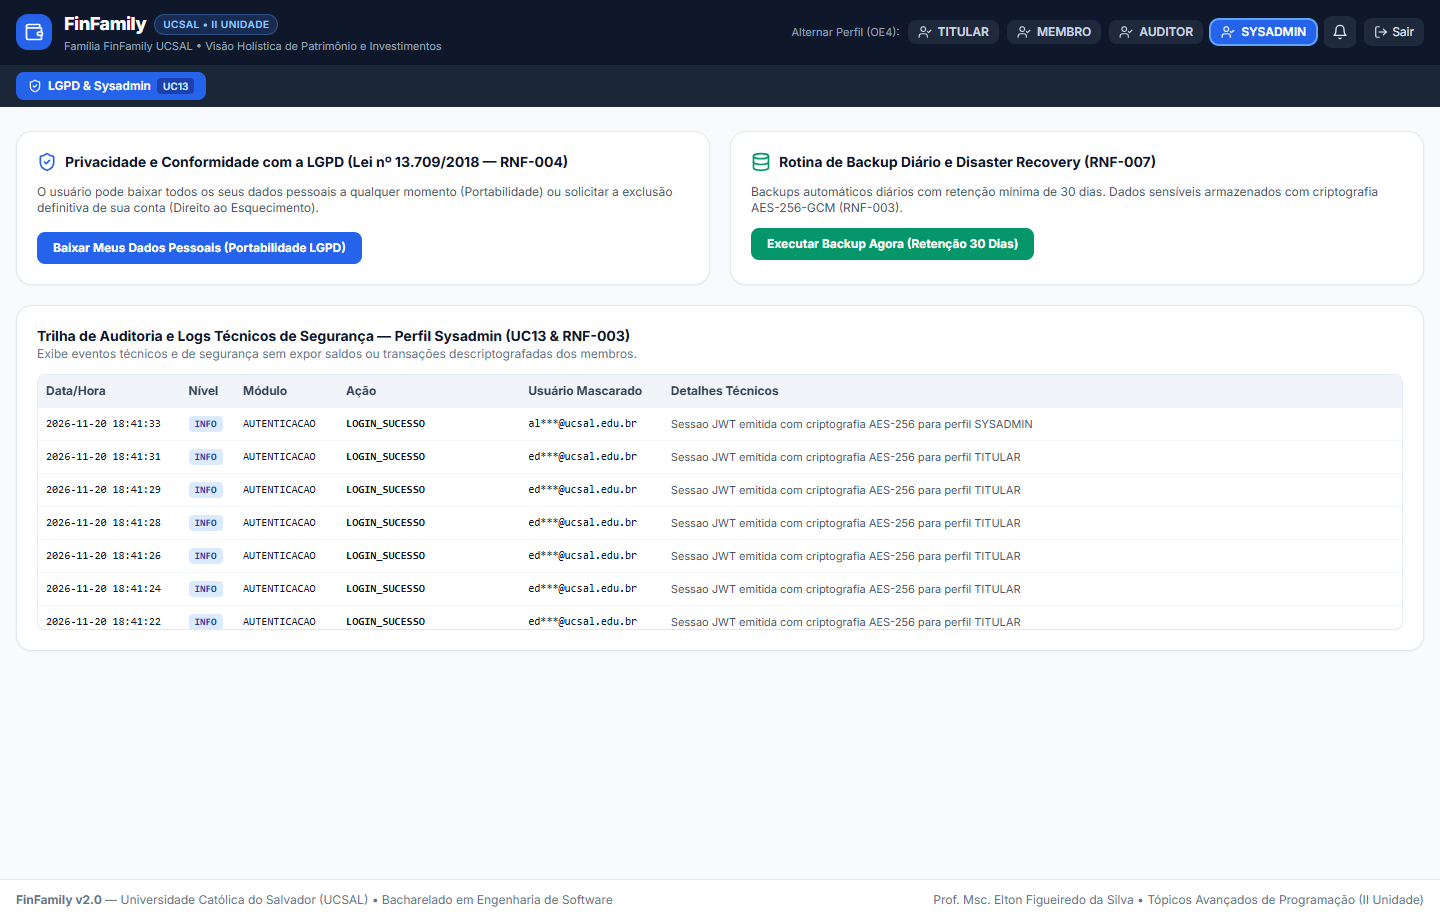
\includegraphics[width=0.95\textwidth]{figuras/tela_10_seguranca_lgpd_sysadmin.png}
    \fonte{Autoria própria (2026).}
\end{figure}

\subsection{Controle de acesso por perfil}

As permissões de cada perfil são garantidas pelo servidor: requisições sem token recebem a resposta 401, e operações não permitidas ao perfil recebem a resposta 403. A interface exibe a cada perfil apenas as ações que ele pode executar e substitui os formulários restritos por um aviso. A Tabela \ref{tab:permissoes} resume as permissões, e as Figuras \ref{fig:auditor} e \ref{fig:membro} mostram a aplicação vista pelo Auditor e pelo Membro.

\begin{table}[H]
\centering
\caption{Permissões por perfil}
\label{tab:permissoes}
\begin{tabularx}{\textwidth}{p{3.2cm}X}
\toprule
\textbf{Perfil} & \textbf{Operações permitidas} \\
\midrule
Titular & Todas as operações do próprio grupo: contas, categorias, orçamentos, membros, investimentos, transações, importação, assistente e exportação. \\
Membro & Leitura dos dados do grupo, lançamento de transações, importação de extratos, uso do assistente e exportação; exclui apenas as transações que lançou. \\
Auditor & Somente leitura dos painéis e relatórios do grupo. \\
Administrador do Sistema & Somente logs técnicos e backup, sem acesso a dados financeiros. \\
Convidado & Somente a resposta ao próprio convite. \\
\bottomrule
\end{tabularx}
\fonte{Autoria própria (2026).}
\end{table}

\begin{figure}[H]
    \centering
    \caption{Perfil Auditor: acesso somente de leitura (OE4)}
    \label{fig:auditor}
    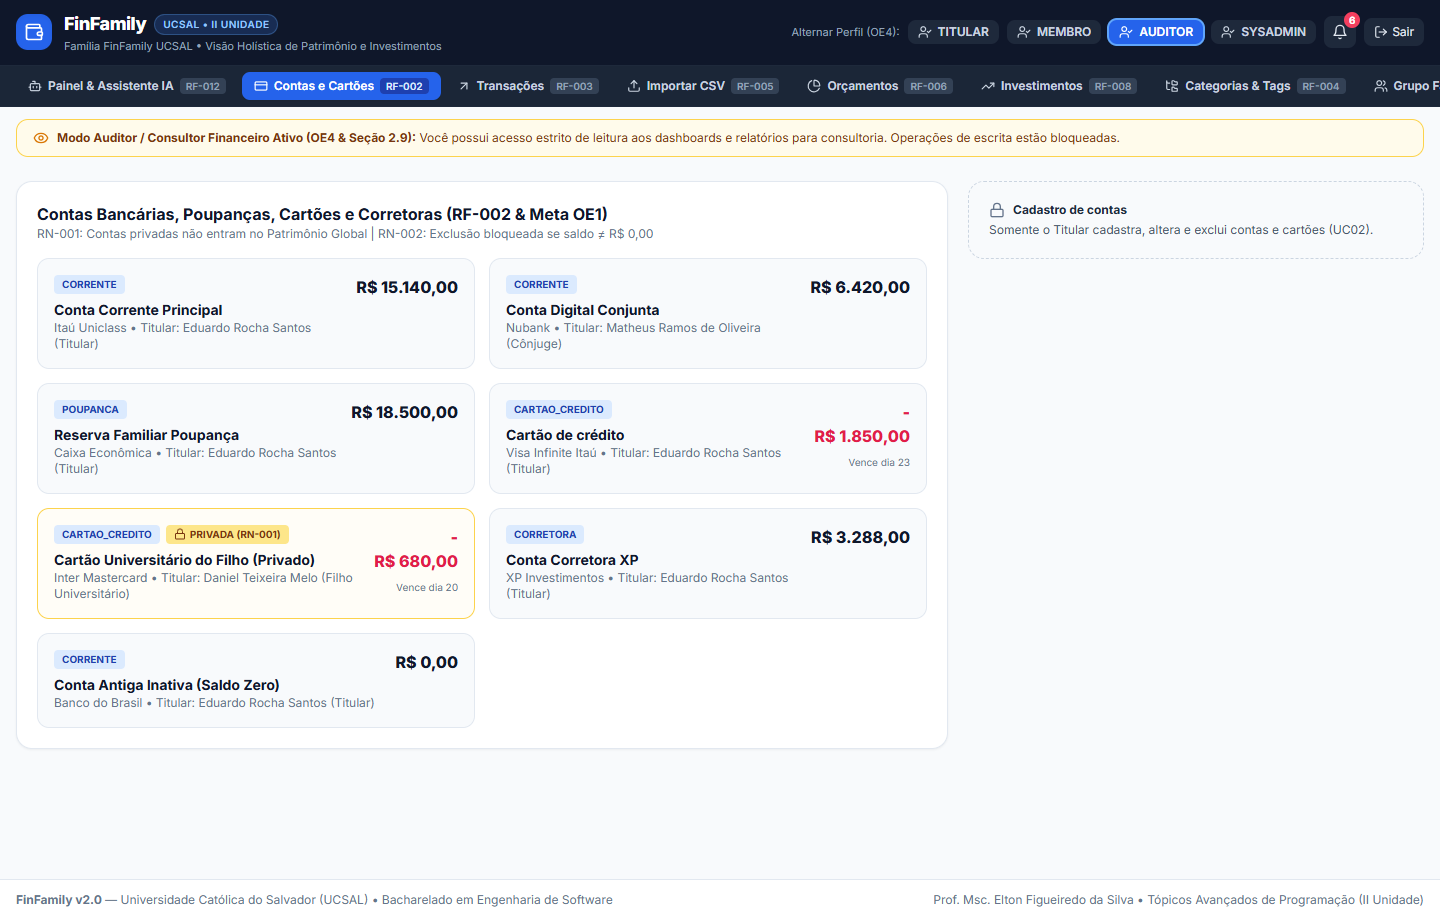
\includegraphics[width=0.95\textwidth]{figuras/tela_11_auditor_somente_leitura.png}
    \fonte{Autoria própria (2026).}
\end{figure}

\begin{figure}[H]
    \centering
    \caption{Perfil Membro: acompanhamento das metas definidas pelo Titular}
    \label{fig:membro}
    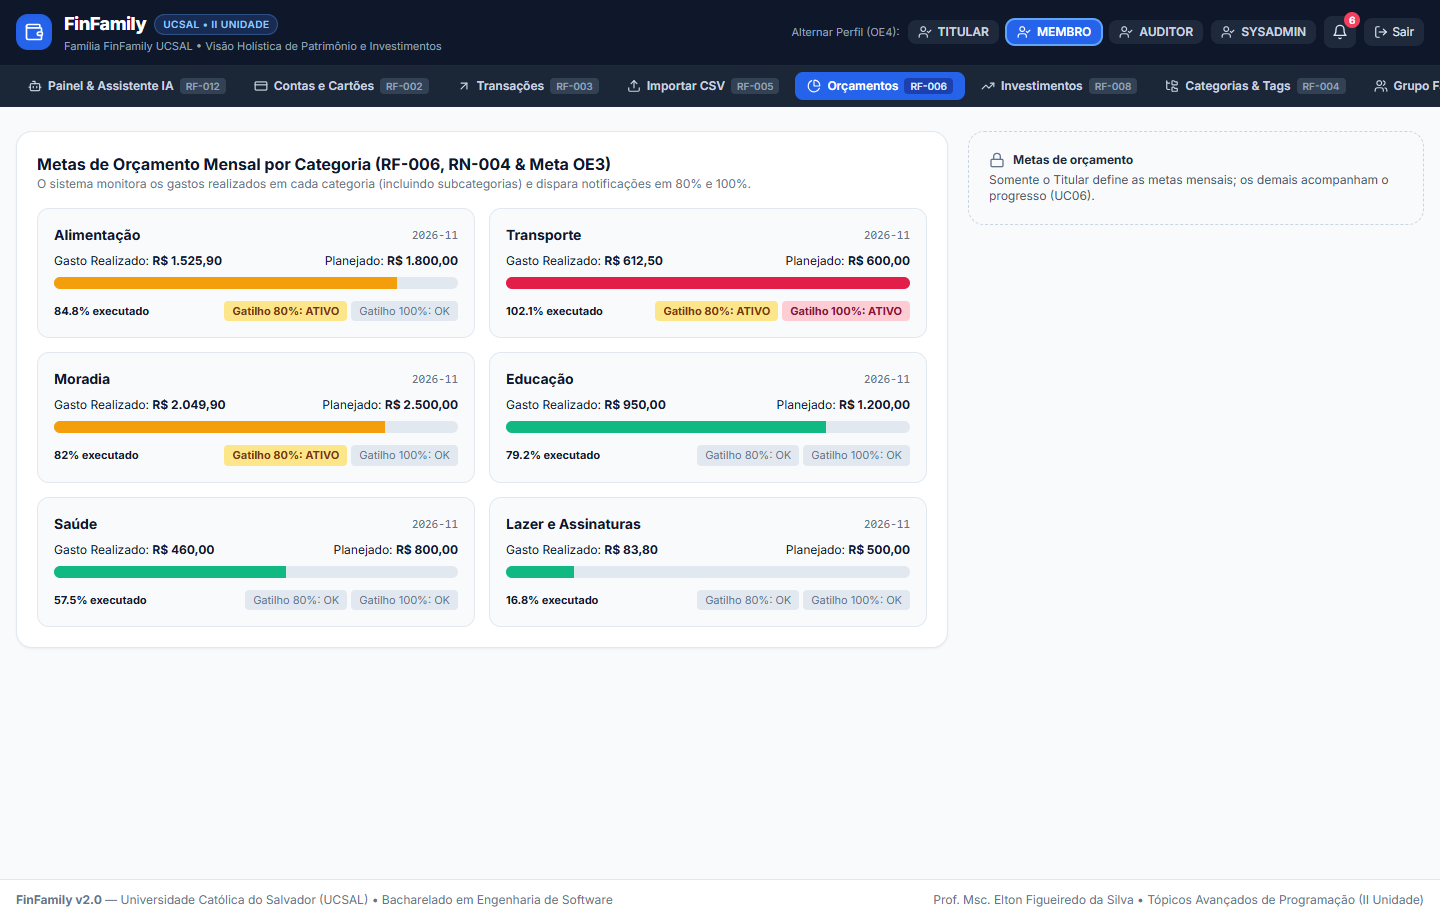
\includegraphics[width=0.95\textwidth]{figuras/tela_12_membro_permissoes.png}
    \fonte{Autoria própria (2026).}
\end{figure}

\subsection{Resposta ao convite}
\label{sec:convite}

Conforme o fluxo BPMN de inclusão de membro, o convidado que ainda não aceitou o convite não visualiza os dados do grupo. Ao entrar no sistema, ele vê a tela da Figura \ref{fig:convite}, onde aceita ou recusa o convite; após o aceite, um novo login libera o acesso conforme o papel definido pelo Titular.

\begin{figure}[H]
    \centering
    \caption{Tela de resposta ao convite (RF-007)}
    \label{fig:convite}
    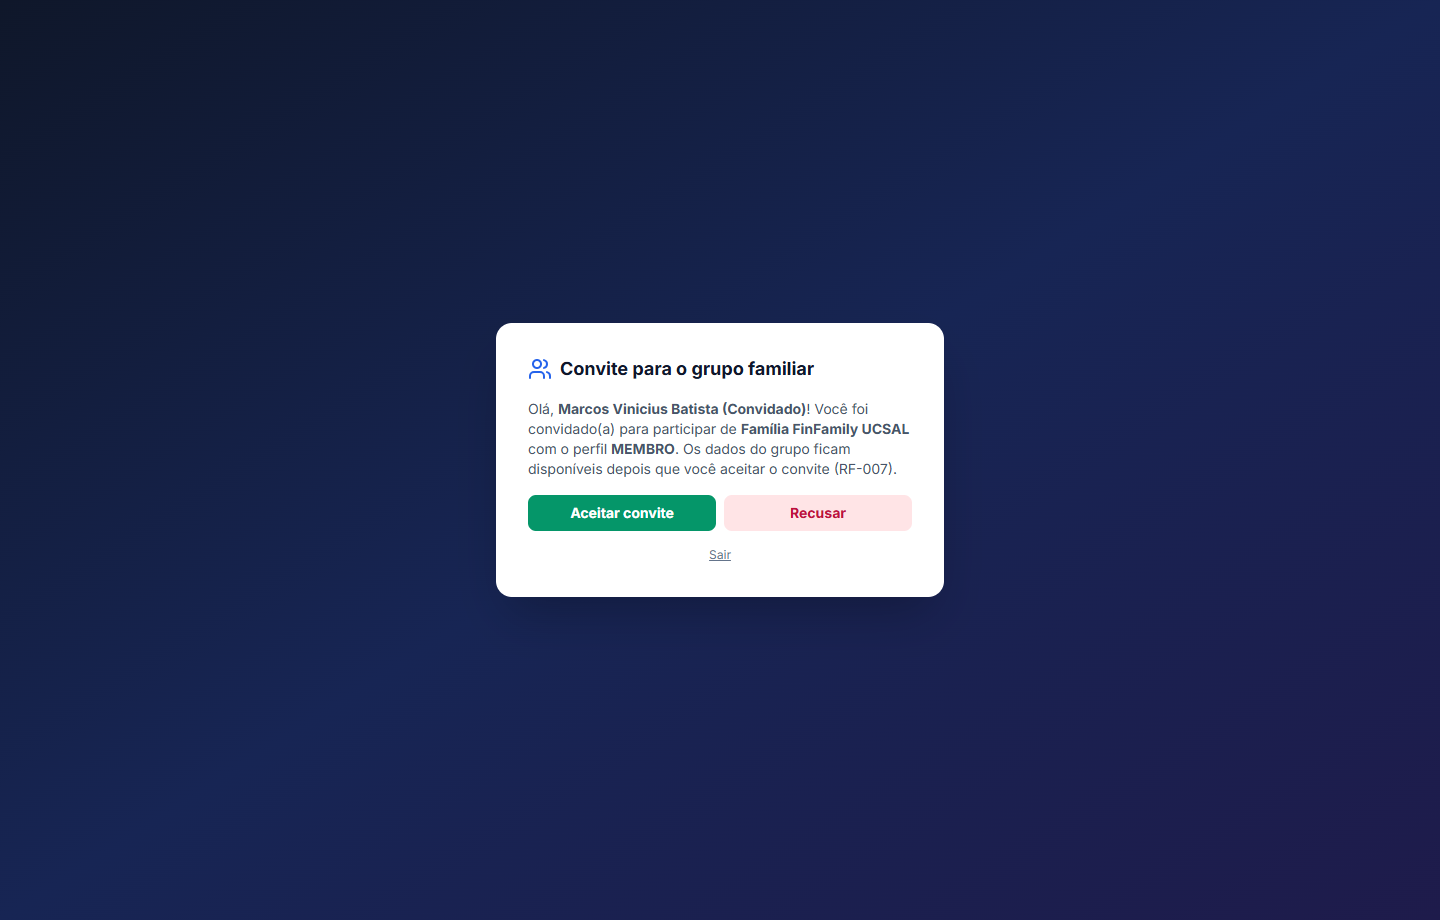
\includegraphics[width=0.95\textwidth]{figuras/tela_13_convite_membro.png}
    \fonte{Autoria própria (2026).}
\end{figure}

\section{Código do Back-End (Item 14)}
\label{sec:codigo}

O servidor segue o modelo de domínio da Unidade I. Os códigos a seguir são trechos do repositório que implementam as regras de negócio, a integração com o modelo de linguagem e o controle de acesso.

\subsection{Privacidade de contas, exclusão e conciliação de extratos}

O método \texttt{patrimonioLiquido()} de \texttt{GrupoFamiliar} ignora as contas privadas (RN-001). Em \texttt{Conta}, o método \texttt{podeSerExcluida()} exige saldo zero (RN-002) e \texttt{gerarHashConciliacao()} gera o \textit{hash} SHA-256 que impede duplicidades na importação de extratos (OE2), conforme o Código \ref{cod:conta}.

\begin{lstlisting}[caption={RN-001, RN-002 e conciliação de extratos (GrupoFamiliar.java e Conta.java)},label={cod:conta}]
public BigDecimal patrimonioLiquido() {
    return contas.stream()
            .filter(c -> !Boolean.TRUE.equals(c.getPrivada()))
            .map(c -> c.getSaldo() != null ? c.getSaldo() : BigDecimal.ZERO)
            .reduce(BigDecimal.ZERO, BigDecimal::add);
}

public Boolean podeSerExcluida() {
    return this.saldo == null || this.saldo.compareTo(BigDecimal.ZERO) == 0;
}

public static String gerarHashConciliacao(Long contaId, LocalDate data, BigDecimal valor, String descricao) {
    String descNorm = descricao == null ? "" : descricao.trim().toLowerCase().replaceAll("\\s+", " ");
    String valorNorm = valor == null ? "0.00" : valor.setScale(2, RoundingMode.HALF_UP).toPlainString();
    String base = (contaId != null ? contaId : 0L) + "|" + data + "|" + valorNorm + "|" + descNorm;
    MessageDigest md = MessageDigest.getInstance("SHA-256");
    return HexFormat.of().formatHex(md.digest(base.getBytes(StandardCharsets.UTF_8)));
}
\end{lstlisting}

\subsection{Alertas de orçamento}

O método \texttt{verificarAlerta()} de \texttt{Orcamento} gera uma notificação quando os gastos atingem 80\% do planejado e outra ao atingir 100\% (RN-004), conforme o Código \ref{cod:orcamento}.

\begin{lstlisting}[caption={Gatilho de 80\% do orçamento (Orcamento.java)},label={cod:orcamento}]
public List<Notificacao> verificarAlerta() {
    List<Notificacao> notificacoes = new ArrayList<>();
    BigDecimal percentual = percentualGasto();
    if (percentual.compareTo(BigDecimal.valueOf(80)) >= 0 && !Boolean.TRUE.equals(this.alerta80Disparado)) {
        this.alerta80Disparado = true;
        Notificacao n80 = new Notificacao();
        n80.setTipo(TipoNotificacao.ORCAMENTO_80);
        n80.setGrupo(this.grupo);
        notificacoes.add(n80);
    }
    // o gatilho de 100% segue a mesma estrutura
    return notificacoes;
}
\end{lstlisting}

\subsection{Integração com o modelo de linguagem}

No \texttt{AssistenteIAService}, o comando é enviado ao modelo de linguagem pelo \texttt{ClienteLLM}, que se comunica com o Google Gemini ou com o Ollama local. A resposta em JSON é convertida em um \texttt{Comando} com valor, descrição, data, conta, categoria, parcelas e período. Se o serviço estiver indisponível, exceder 3 segundos ou devolver uma resposta inválida, o motor local assume (Código \ref{cod:ia}). Antes de gravar um lançamento, o serviço exige a confirmação do usuário (RN-006).

\begin{lstlisting}[caption={Interpretação pelo modelo de linguagem, contingência e RN-006 (AssistenteIAService.java)},label={cod:ia}]
String promptSeguro = montarPromptSeguroRnf004(texto, contas, categorias);

Comando comando = clienteLLM.gerarJson(promptSeguro)
        .map(r -> converterRespostaLLM(r.json(), r.provedor(), texto, contas, categorias))
        .orElse(null);

if (comando == null) {
    comando = interpretarMotorNlpHibrido(texto, contas, categorias);
    comando.setProvedorIA(PROVEDOR_CONTINGENCIA);
}

if ("registrar".equalsIgnoreCase(comando.getIntencao()) && !confirmadoPeloUsuario) {
    throw new IllegalStateException(
            "RN-006 Violada: Um lançamento interpretado pelo assistente de IA só pode ser gravado após o usuário confirmar o card exibido.");
}
\end{lstlisting}

\subsection{Controle de acesso por perfil}

A classe \texttt{SecurityConfig} exige o token JWT em toda a API e define o que cada perfil pode acessar (Código \ref{cod:seguranca}). A classe \texttt{ControleAcesso} complementa essas regras ao verificar se o registro solicitado pertence ao grupo familiar do usuário, cujo identificador é lido do próprio token.

\begin{lstlisting}[caption={Regras de acesso por perfil (SecurityConfig.java)},label={cod:seguranca}]
.requestMatchers(HttpMethod.POST, "/api/auth/login", "/api/auth/register").permitAll()
.requestMatchers("/api/sysadmin/**").hasRole(SYSADMIN)
.requestMatchers(HttpMethod.GET, "/api/exportacao/**").hasAnyRole(TITULAR, MEMBRO)
.requestMatchers(HttpMethod.GET, "/api/**").hasAnyRole(TITULAR, MEMBRO, AUDITOR)
.requestMatchers(HttpMethod.POST, "/api/transacoes", "/api/importacao/**",
        "/api/assistente/**").hasAnyRole(TITULAR, MEMBRO)
.requestMatchers("/api/**").hasRole(TITULAR)
\end{lstlisting}

\subsection{Criptografia de dados sensíveis}

Para atender ao RNF-003, a classe \texttt{AesAttributeConverter} criptografa os dados sensíveis com AES-256 no modo GCM, utilizando um vetor de inicialização aleatório a cada gravação (Código \ref{cod:aes}).

\begin{lstlisting}[caption={Criptografia AES-256-GCM (AesAttributeConverter.java)},label={cod:aes}]
public static String encrypt(String plainText) {
    byte[] iv = new byte[IV_LENGTH_BYTE];
    new SecureRandom().nextBytes(iv);
    Cipher cipher = Cipher.getInstance(ALGORITHM);
    GCMParameterSpec parameterSpec = new GCMParameterSpec(TAG_LENGTH_BIT, iv);
    cipher.init(Cipher.ENCRYPT_MODE, getKey(), parameterSpec);
    byte[] cipherText = cipher.doFinal(plainText.getBytes(StandardCharsets.UTF_8));
    // o IV e o texto cifrado sao gravados juntos, em Base64
}
\end{lstlisting}

\section{Verificação dos Resultados}
\label{sec:validacao}

Os testes automatizados foram executados com JUnit 5 por meio do comando \texttt{mvnw.cmd test}, com 33 testes aprovados e nenhuma falha. Eles estão organizados em cinco classes: \texttt{FinFamilySystemTests}, com as regras de negócio; \texttt{FinFamilyApiAndPerformanceTests}, com a API e a latência; \texttt{AssistenteIALlmTests} e \texttt{ClienteLLMTests}, com a integração com o modelo de linguagem e a contingência; e \texttt{ControleAcessoTests}, com 12 cenários de permissão por perfil e de isolamento entre grupos familiares. A Tabela \ref{tab:resultados} compara os resultados com as metas da Unidade I.

\begin{table}[H]
\centering
\caption{Resultados da Unidade II em relação às metas da Unidade I}
\label{tab:resultados}
\begin{tabularx}{\textwidth}{p{1.1cm}p{4.2cm}p{3.6cm}X}
\toprule
\textbf{ID} & \textbf{Objetivo} & \textbf{Meta} & \textbf{Resultado} \\
\midrule
OE1 & Centralizar as contas da família & 4 tipos de conta & Atendido: 4 tipos implementados e testados \\
OE2 & Importar extratos sem duplicidade & 0 duplicidades & Atendido: 0 duplicidades com \textit{hash} SHA-256 \\
OE3 & Controlar o orçamento com alertas & Alertas em 80\% e 100\% & Atendido em todos os casos de teste \\
OE4 & Colaboração com segurança & Perfis com permissões distintas & Atendido: permissões garantidas no servidor e verificadas em 12 testes \\
OE5 & Assistente de IA & $\ge$ 80\% de 50 comandos em menos de 3 s & Atendido: 50 de 50 corretos, média de 610 ms (24 pelo Gemini e 26 pela contingência) \\
OE6 & Entregar o MVP & 12 requisitos funcionais & Atendido: 12 RFs, 6 RNs e 7 RNFs implementados \\
\bottomrule
\end{tabularx}
\fonte{Autoria própria (2026).}
\end{table}

\section{Vídeos Individuais (Item 15)}
\label{sec:videos}

Cada desenvolvedor da equipe gravou um vídeo explicando o desenvolvimento do projeto, conforme a Tabela \ref{tab:videos}.

\begin{table}[H]
\centering
\caption{Vídeos individuais dos desenvolvedores}
\label{tab:videos}
\begin{tabularx}{\textwidth}{p{6cm}X}
\toprule
\textbf{Integrante} & \textbf{Link do vídeo} \\
\midrule
Alexandre Villarino e Silva & \url{https://youtu.be/4GROkspWBvE} \\
Daniel Teixeira Melo & \url{https://youtu.be/ax9L6RPY5Yo} \\
Eduardo Rocha Santos & \url{https://youtu.be/bbYyIgs7PJo} \\
Marcos Vinicius Sousa Batista & \url{https://www.youtube.com/watch?v=BCikNz2T5Fg} \\
Vinicius Freitas de Oliveira Souza & \url{https://www.youtube.com/watch?v=3ZGFuRa-kxw} \\
\bottomrule
\end{tabularx}
\fonte{Autoria própria (2026).}
\end{table}

\section{Conclusão}

A Unidade II transformou em software a especificação e a modelagem da Unidade I. A arquitetura em três camadas, com Java 21 e Spring Boot no servidor, React na interface e banco de dados relacional, permitiu implementar os doze requisitos funcionais, as seis regras de negócio e os sete requisitos não funcionais. O assistente conversacional utiliza um modelo de linguagem para interpretar os comandos e mantém o funcionamento por meio de um motor local quando o serviço externo está indisponível. O controle de acesso por perfil, aplicado no servidor, garante que cada usuário execute apenas as operações previstas para o seu papel.

Como trabalhos futuros, a equipe aponta o uso de um plano pago ou de um modelo local para reduzir o uso da contingência, a migração do banco de dados para PostgreSQL em produção e a geração automática das transações recorrentes.

\bibliography{referencias}

\end{document}
